\documentclass[conference]{IEEEtran}
% generated by Docutils <http://docutils.sourceforge.net/>
\usepackage{fixltx2e} % LaTeX patches, \textsubscript
\usepackage{cmap} % fix search and cut-and-paste in Acrobat
\usepackage{ifthen}
\usepackage[T1]{fontenc}
\usepackage[utf8]{inputenc}
\usepackage{float} % float configuration
\floatplacement{figure}{H} % place figures here definitely
\usepackage{graphicx}

%%% Custom LaTeX preamble
% PDF Standard Fonts
\usepackage{mathptmx} % Times
\usepackage[scaled=.90]{helvet}
\usepackage{courier}
\usepackage{graphicx}
\usepackage{amsmath}
\usepackage{tabularx}
\usepackage{multirow}
\bibliographystyle{IEEEtran}

%%% User specified packages and stylesheets

%%% Title Data
\title{Comparative API Complexity Analysis of Two Platforms for Networked Multiplayer Games}
\author{
  \IEEEauthorblockN{
    Toni Alatalo\IEEEauthorrefmark{1}\IEEEauthorrefmark{2}
    Erno Kuusela\IEEEauthorrefmark{1}\IEEEauthorrefmark{2} 
    Rauli Puuperä\IEEEauthorrefmark{1}\IEEEauthorrefmark{2}
    and Timo Ojala\IEEEauthorrefmark{1}
  }
  \IEEEauthorblockA{\IEEEauthorrefmark{1}Department of Computer Science and Engineering, University of Oulu}
  \IEEEauthorblockA{\IEEEauthorrefmark{2}Playsign Ltd., Oulu, Finland}
}
\date{}

%%% Body
\begin{document}
\maketitle
\begin{abstract}

In this paper we focus on characterizing the complexity of an API to
understand how gaming platform APIs succeed in easing the development
of networked multiplayer games. We first present an open source tool
for automatic quantitative assessment of the complexity of a software
API by analyzing a source code using the API with Sneed's Object-Point
(OP) method. We then apply the tool to compare the APIs of two
platforms for networked multiplayer games, the open source realXtend
Tundra SDK and the proprietary Union, using pre-existing
implementations of the Pong game atop the two platforms as reference
games. Our findings show that the tool successfully quantifies the
different amounts of complexity that are due to the different design
rationale of the platforms.

\end{abstract}

\section{Introduction%
  \label{introduction}%
}

Programming distributed networked applications is generally more
complex than developing standalone software. Developer typically needs
to deal with events, conflicts and error conditions originating from
other parts of the distributed system as well as the local user. This
is emphasized in multiuser real-time systems when compared to the
relatively leisurely request-response interaction patterns of most
client-server applications. Developing a massively multiplayer online
game (MMOG) has been estimated to typically take two to three times
longer than creating and launching a single-player game \cite{middleware}.

A common approach to ease application development are higher level
software abstractions, such as networking libraries simplifying
connection management and messaging, and distributed object systems
automating remote calls and data synchronization. For an application
developer, these resources are provided as a set of abstractions
constituting the application programming interface (API). It has been
noted how making good APIs is hard - and that creating a bad API is
easy \cite{api-matters}. Even a small quirk in an API can accumulate
to substantial problems in larger bodies of application source
code. API design has a significant impact on software quality, and
increased API complexity is associated with increased software failure
rates \cite{cmu-api_failures}.

The underlying motivation of our study is to understand how the API of
the open source realXtend Tundra SDK (Tundra from now on), recently
introduced by Alatalo \cite{Alatalo2011}, succeeds in hiding the
complexity of developing networked multiplayer games. Tundra strives
to adopt the best design practices from game engine literature,
notably aggregation using an abstract entity-component model. The
objective of the entity-component model and the whole Tundra platform
is to make development of networked multiplayer games easy and
productive. Specifically in terms of networking, Tundra features
attribute autosynchronization, a simple form of transparent remote
procedure calls (entity actions) and efficient customized movement
messages with inter- and extrapolation logic (dead reckoning).

Rigorous quantitative assessment of a gaming platform in terms of ease
and productivity of development is very challenging. Hsiao and Yuan
\cite{middleware} proposed four essential ``ease of'' requirements for a MMOG
middleware: ease of development, deployment, maintenance and
change. However, they noted the difficulty of quantitatively measuring
for example the ease of development or change, and focused only on
platform scalability in their evaluation. 

In this paper we quantify the “ease of” dimension as an inverse
function of the complexity of the software API used for game
development. Inspired by recent progress in quantitative techniques
for software complexity analysis
\cite{cmu-api_failures,api-complexity-analysis}, we first propose a
tool for automated quantitative assessment of the complexity of a
software API based on automatic analysis of the source code using the
API with Sneed’s Object-Point (OP) method. Then we use the tool to
compare Tundra’s API complexity to that of the Union platform with
pre-existing implementations of the Pong game on the two platforms,
i.e. Pong serves as the minimal reference of a networked multiplayer
game in our study. Our data shows that the tool indeed successfully
quantifies the different amounts of complexity that the game developer
has to manage on these two alternate platforms.

This paper is organized as follows. After briefly reviewing related
work on API complexity analysis we present our tool. Then we report
our case study on using the tool to compare the API complexity of the
two platforms in the development of the Pong game. We conclude the
paper with a discussion on various aspects of the study.


\section{Related Work on API Complexity Analysis%
  \label{related-work-on-api-complexity-analysis}%
}

A wide range of qualitative and quantitative approaches have been
proposed for assessing the complexity of software APIs. The API
usability research has adapted traditional qualitative usability
evaluation methods of the HCI field such as thinking aloud, heuristic
evaluation and cognitive walkthroughs into evaluating APIs
\cite{overview}. Employed metrics include the completion times of
predefined tasks, for example. In comparison to task-based usability
evaluation of GUIs, API evaluation based on human observations is
challenging. When developing a small application can take even weeks,
fitting valid evaluation tasks into an observation session lasting
typically 1-2 hours is difficult \cite{conceptmaps}. The recently
introduced peer review \cite{apipeerreview} and the concept maps
\cite{conceptmaps} methods address this problem by involving real world
usage of an API over a long period of time. However, they are still
considerably laborious and yield only qualitative findings.

Recently, statistical (quantitative) methods have been proposed for
analysing the complexity of software APIs. Cataldo and de Sousa
\cite{cmu-api_failures} studied two large corporate software projects
and nine open source projects and found a link between the API
complexity and the failure proneness of the software quantified by the
number of bug reports from the field. They quantified the complexity
of an API by simply calculating the number of public methods and
attributes. That approachs is subject to severe limitations as it
fails to take into account pre- and post-invocation assumptions and
possible invocation sequences.

de Souza and Bentolila \cite{automatic-api-eval} introduced the Metrix tool
that evaluates an API by calculating Bandi’s software metrics for
interface size, interaction level and operation argument complexity
from the API specification. After analysing eleven different APIs with
the Metrix tool, de Souza and Bentolila concluded that calculating
such simple metrics directly from the API specification can produce
misleading results. A more complete API may appear more complex, even
if it provides good abstractions that allow completing a particular
task at hand with only a small subset of the API.

An alternative to evaluating the complexity of an API with simple
metrics calculated from the API specification is to assess the
complexity of programs developed using the API. Sobernig et
al. \cite{api-complexity-analysis} proposed exactly this in their
comparative study of the complexity of four different API designs. To
characterize the complexity of a particular API, they applied Sneed’s
\cite{Sneed} Object-Point (OP) analysis to a software realized atop the
API. The key is to apply a surrogate measurement so that a program
developed using an API is analyzed, not the API specification itself.


\section{Tool for Automated Analysis of API Complexity%
  \label{tool-for-automated-analysis-of-api-complexity}%
}

Our first task was to develop a tool that facilitates automated and
quantitative evaluation of the complexity of an API from an existing
body of source code developed using the API. Such a tool would come
with several advantages. First, real world data, i.e. source codes of
existing applications, could be utilized. Second, in comparison to
manual methods the analysis would be quick with immediate feedback and
would require only a limited amount of human labor. Third,
longitudinal studies of API development would be straightforward to
conduct by analysing successive software versions. A fully automated
analysis could be embedded into the continuous integration of a
software bundle, to characterize the evolution of its complexity over
time.

Following the work of Sobernig et al. \cite{api-complexity-analysis}, we
base our tool on Sneed’s Object-Point (OP) method \cite{Sneed}. However, in
contrast to their manual data collection, our tool automatically
extracts the data needed by the OP method from a program’s source
code. The OP method uses intermediate UML models as the data to
compare programs in different languages. Importantly, the OP method
allows direct tracking between indicator values and program
structures, which is elementary in evaluating API designs. For
example, if many codebases get a high proportion of their complexity
value due to a specific part of an API, it can then be examined
qualitatively. So called API hotspots and coldspots have been
previously automatically mined from source code \cite{spotweb}. There,
however, the specific parts of an API are not analyzed as sources of
complexity, but simply to identify how much they are used. Their
source code mining is similar to our tool that also needs to identify
which functions are called and how often to employ the OP method.


\subsection{Sneed's Object-Point (OP) method%
  \label{sneed-s-object-point-op-method}%
}

Although the OP method was originally developed for deriving early
work estimates from UML design diagrams, recently it has been applied
to analysing the complexity and cost of existing software
implementations. While the early COCOMO software cost models used
simply program size (LOC, lines of code) to estimate development
effort, later the more versatile Function-Point, the Data-Point and
finally the Object-Point methods have emerged to incorporate
functionality and other program properties into the cost estimate
\cite{henrich97repositorybased}.

Sobernig \emph{et al.} illustrated the relative robustness of the OP method
to the simple LoC (lines of code) metric on two software
implementations. The first software had only 48 LoC but resulted in
356.34 OP. The second software had 144 LoC but only 266.76 OP. Their
reasoning was: \emph{``an API user is only exposed to an API feature chunk
of low structural complexity''}, as the chunk's \emph{``size is limited in
terms of participating classes and the smallest number of operations
per class''} and it \emph{``shows a relatively weak connectedness of classes,
resulting from the small number of associations and generalizations
between the classes''}. This reasoning is of utmost relevance to our
objective of easing the development of networked game development with
good API designs. We pursue a limited set of powerful abstractions
with clear interactions that a game developer could easily learn and
grow to master. Not all source code lines are equal - a poorly
designed API makes it a struggle to get even a few operations working
if the developer has to strive for functionality scattered around in
an incoherent way.

The Object-Points, as applied here, are a sum of two parts: Class
Points (CP) and Message Points (MP).

\textbf{Class Points (CP)} (Eq. 1-4) are calculated from the static class structure: the
class count and sums of attribute, operation and relation
counts. Weights are employed to correct the values for the overall
calculation. Class inheritance is taken into account by calculating
novelty weights for specializing classes.

\textbf{Message Points (MP)} (Eq. 5-8) are defined by the set of operations
(functions/methods) \emph{actually used} in the software. First, the number
of operations is recorded. Then, the parameter count for each called
operation is collected. Also, the source and target counts of the
operation calls are established. Again, novelty weights are used to
compensate for repeated occurrences due to subclassing.

\small
\begin{align}
CP &= \left(W_C |C| + \sum_{c_ \in C} |A_c| + W_{R_C} \sum_{c \in C} |R_c| + W_{O_C} \sum_{c \in C} |O_c| \right) \overline{N_C},\\ &\text{where}\\
\overline{N_C} &= \frac{\sum_{c \in C} N_c}{|C|},\, \text{and}\\
N_c &=
\begin{cases}
1,& \text{if class is novel}\\
0.5,& \text{if class has a super class}\\
\end{cases}
\end{align}
\begin{align}
MP &= \left(W_{O_M} |O_M| + \sum_{o \in O_M} |P_o| + W_{S_O} \sum_{o \in O_M} |S_o| + W_{T_O} \sum_{o \in O_M} |T_o| \right) \overline{N_{O_M}},\\ &\text{where}\\
\overline{N_{O_M}} &= \frac{\sum_{o \in O_M} N_o}{|O_M|},\,\text{and}\\
N_o &=
\begin{cases}
1,& \text{if operation is novel}\\
0.5,& \text{if operation is provided by super class}\\
\end{cases}
\end{align}

\begin{tabularx}{\linewidth}{rX}
\hline
$C, |C|...$ & Set of classes, Class count \\
$|A_c|...$  & Attribute count per class   \\
$|O_c|...$  & Operation count --''--      \\
$|R_c|...$  & Relation count --''--       \\
$N_c...$    & Novelty weight of class c \\
$\overline{N_C}$ & Avg. class novelty \\
$|O_M...$  & Set of called operations \\
$|O_M|...$ & Called operation counts \\
$|P_o|...$ & Parameter count of operation o \\
$|S_o|...$ & Source count --''-- \\
$|T_o|...$ & Target count --''-- \\
$N_o...$   & Novelty weight --''-- \\
\end{tabularx}
\normalsize

The weights are adopted directly from the earlier usage of OP for API
complexity analysis, which further uses the standard Data Points
analysis values by Sneed. Please see \cite{api-complexity-analysis} for a
detailed description of the calculation of the CP and MP values.


\subsection{Extracting Object-Point data from source code%
  \label{extracting-object-point-data-from-source-code}%
}

To obtain the static class data for the Class Points (CP), we utilize
existing source code parsing and annotation systems in the API
documentation tools. The first alternative implementations for a
minimal networked game on different modern high-level APIs studied
here are written as a Javascript application and a combination of
Actionscript (as3) for the client and Java for the server module. We
have developed parsers for the internal / intermediate representations
of class and method signatures in JsDoc JSON and AsDoc XML
formats. The class information is read by a Python application to an
internal model which contains the data for the OP calculation,
implemented in another module in the same Python application.

To calculate the Message Points reflecting the \emph{dynamic function
calls}, we use the Closure Javascript compiler to traverse the source
code to collect function calls and their argument counts.  A parser
made with Python is used to read the function call data required to
calculate the MPs.

While our tool calculates complete Class Point data, it currently
omits two factors in Message Point data: the source and target counts
of the interactions, and the novelty weight. While the tool tallies
separate calls to each called function in the source code, it is not
yet clear how to map them into the MP values. In Sobernig \emph{et al.} the
source and target counts were always set to 1. For the novelty weight
we should check for each called operation called whether it is
implemented in that class or inherited from a superclass. Our tool
does not currently know the class of the object in which an operation
is called. These omissions are not expected to affect the OP values
significantly, at least not enough to affect the conclusions of this
study.

Finally, to facilitate manual validation and visual communication of
the data extracted from the source codes, our tool also creates UML
class diagrams from the very same in-memory data structure that is
used in the OP calculation. We chose the UXF format of the open source
Umlet GUI diagram tool, due to its simple and straightforward XML
format and the even simpler plaintext syntax used to describe
individual UML elements, such as a class or a relation. This allows
further manual editing of the diagrams with the GUI tool to improve
the layout and annotation with notes.

Repository based automatic queries for OP analysis have been presented
earlier by Henrich \cite{henrich97repositorybased}. There a repository of
documents, or abstract software design models (PCTE), were queried
using the P-OQL language. We are not aware of any previous
implementation of directly extracting data for the OP method from the
source code.


\section{Case Study in API Complexity Analysis%
  \label{case-study-in-api-complexity-analysis}%
}


\subsection{Pong as reference game%
  \label{pong-as-reference-game}%
}

We propose using the Pong game as a minimal networked multiplayer
reference game in the subsequent API complexity analysis. While Pong
is tiny in its functionality, it is still sufficient for demonstrating
key challenges in networked games, given the functional combination of
the clients controlling their own paddles and the ball bouncing in the
shared space. Pong has been used in networked game research earlier,
recently in an interesting study of latency compensation techniques
\cite{pong-ping}. Also even a minimal game suffices to reveal the amount of
software needed for the basic functionality: launching the networked
software, establishing connections, handling players joining in and
dropping out, and synchronizing gaming events.


\subsection{Game platforms under comparison%
  \label{game-platforms-under-comparison}%
}

In this section we briefly introduce the two game platforms whose API
complexity we are going to compare, the open source realXtend Tundra
SDK \cite{Alatalo2011} and the Union, a proprietary closed source
product\footnotemark[1]. Both are relatively high-level
platforms for networked games and bear several interesting
similarities and differences for this study. Both are specifically
designed for networking, which is exposed to the developer at an
abstract application level. That is, the developer and the game do not
have know anything about sockets or network hosts. Instead, an
abstract container object is provided (Room in Union, Scene in Tundra)
and the game application logic listens to events from the container,
for example when a new client joins the shared session/space. Also,
both platforms provide an automated mechanism for synchronizing shared
state over network. The shared state is stored in special attributes
(objects of type Attribute) residing in the container (in Union
directly in the Room object, in Tundra in the Components of the
Entities in a Scene). The attributes are automatically shared among
all participants, and notifications are provided for parties that have
subscribed to be notified of changes. This way it is simple to for
example set the game scores on the server, and show it in the client
GUIs.

\footnotetext[1]{http://www.unionplatform.com/}

However, the two platforms also have fundamental differences and we
discuss how they manifest in the implementation of the Pong
game. TundraPong\footnotemark[2] was implemented by the leading author of this
paper and an independent developer in two sessions totaling about six
hours. UnionPong\footnotemark[3] was downloaded from the Union website, where it
is available as a tutorial example. While TundraPong is a script
running atop the Tundra platform, UnionPong is a client application,
to which networking functionality has been added by using Union's
Reaktor Flash library. TundraPong utilizes a complete static scene
datafile, where the game logic moves objects around. It runs on an
existing client-server system, and utilizes several default components
of the platform, most notably the data defining visual appearance and
spatial instantiation and movement. In contrast, UnionPong not only
has code to create the appearance of the game court (as it is called
in Court.as), but also to define the data required for the spatial
movement of an object (PongObject has x, y, direction, speed, width
and height). In TundraPong, the predefined built-in Placeable
component contains the position and the Rigidbody component contains
shape information for collisions and speed vector for movement.

\footnotetext[2]{\text{https://github.com/realXtend/doc/tree/master/netgames/PongMultiplayer}}
\footnotetext[3]{\text{http://www.unionplatform.com/?page\_id=1229}}

Thus, it is clear from the offset that UnionPong is more complex, due
to the game code containing a much larger proportion of the
implementation of the functionality. The upcoming API complexity
analysis is still useful as it helps to answer the questions at
hand: a) how the two APIs succeed in hiding the complexity from the
developer and b) how our tool succeeds in evaluating the relative
complexity of the two APIs.


\subsection{Object-Point Data%
  \label{object-point-data}%
}

The OP data of the two Pong implementations is presented in
Table 1. As anticipated, TundraPong has clearly smaller OP values.

For TundraPong the OP data is extracted from the single Javascript
source file (assets/game.js) that contains both client and server
functionality in two respective classes, with GUI and minimal game
session management. UnionPong has separate client and server source
code files in different languages using different
libraries. Therefore, to facilitate more equal comparison, for
TundraPong we also provide the OP data for the client only, even
though it is included in the same source code file.

For UnionPong the OP data is calculated for all 14 client side
ActionScript files and for selected 8 classes related to networking
(GameManager, GameStates, KeyboardController, PongClient, PongObject,
RoomAttributes, RoomMessages, UnionPong). The excluded classes cover
GUI, the 2d scene implementation and general settings and utilities
(clamp, ClientAttributes, Court, HUD, Rectangle and
Settings). KeyboardController is included because it sends remote
control messages from the player to the server (modifies
client.paddle's attributes and says client.commit()).

UnionPong’s Java server component (PongRoomModule.java) contains two
classes: PongRoomModule (implements Module, Runnable) and PongObject,
which is basically a duplicate of the same class in the client. As our
OP data extraction tool does not yet support Java, we collected the OP
data from the server component manually.

\begin{table}[!t]
%% increase table row spacing, adjust to taste
\renewcommand{\arraystretch}{1.3}
% if using array.sty, it might be a good idea to tweak the value of
% \extrarowheight as needed to properly center the text within the cells
\caption{Object-Point data for the two Pong Implementations}
\label{table_example}
\centering
%% Some packages, such as MDW tools, offer better commands for making tables
%% than the plain LaTeX2e tabular which is used here.
\begin{tabular}{|c|c|c|c|c|c|}
\hline
\multirow{2}{*}{metric} & \multicolumn{2}{c|}{Tundra Pong} & \multicolumn{3}{c}{Union Pong}\tabularnewline
\cline{2-6}
& Full & Client only & \multicolumn{1}{c||}{Client Full} & Client Net & Server\tabularnewline
\hline
LoC     & 361 & 115 & 565 & 420 & 281 \\
$|C|$   & 2   & 1   & 14  & 8   & 2   \\
CP      & 75  & 27  & 180 & 140 & 75  \\
MP      & 103 & 63  & 196 & 175 & 87  \\
OP      & 178 & 90  & 376 & 315 & 162 \\
\hline
\end{tabular}
\end{table}

% 20 4 51 1
% OP 178 = CP 75 + MP 103
% 
% 7 2 18 1
% OP 90 = CP 27 + MP 63
% 
% 67 22 135 0.807692307692
% OP 376 = CP 180 + MP 196
% 
% 44 20 96 0.875
% OP 315 = CP 140 + MP 175
% 
% 37 6 57 0.75
% OP 162 = CP 75 + MP 87
% 
% without params in MP calc:
% 
% 67 22 135 0.807692307692
% OP 316 = CP 180 + MP 136
% 
% 44 20 96 0.875
% OP 264 = CP 140 + MP 124


\subsection{UML Diagrams%
  \label{uml-diagrams}%
}

Figures 1 and 2 show the UML diagrams generated from the OP data by
our tool for subsequent manual verification of the analysis and the
API complexity.
\begin{figure}
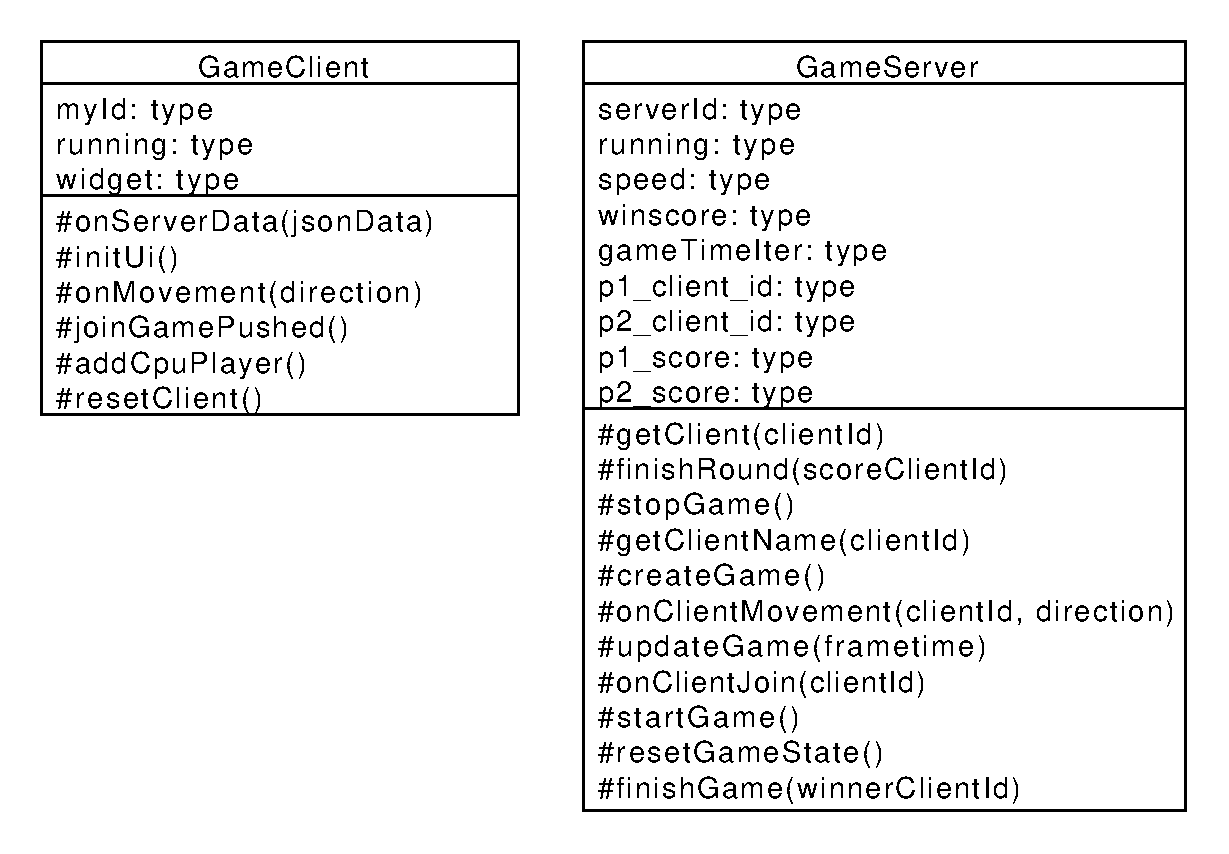
\includegraphics[scale=0.400000]{pics/TundraPong.pdf}
\caption{The two classes in TundraPong game.js.}
\end{figure}
\begin{figure}
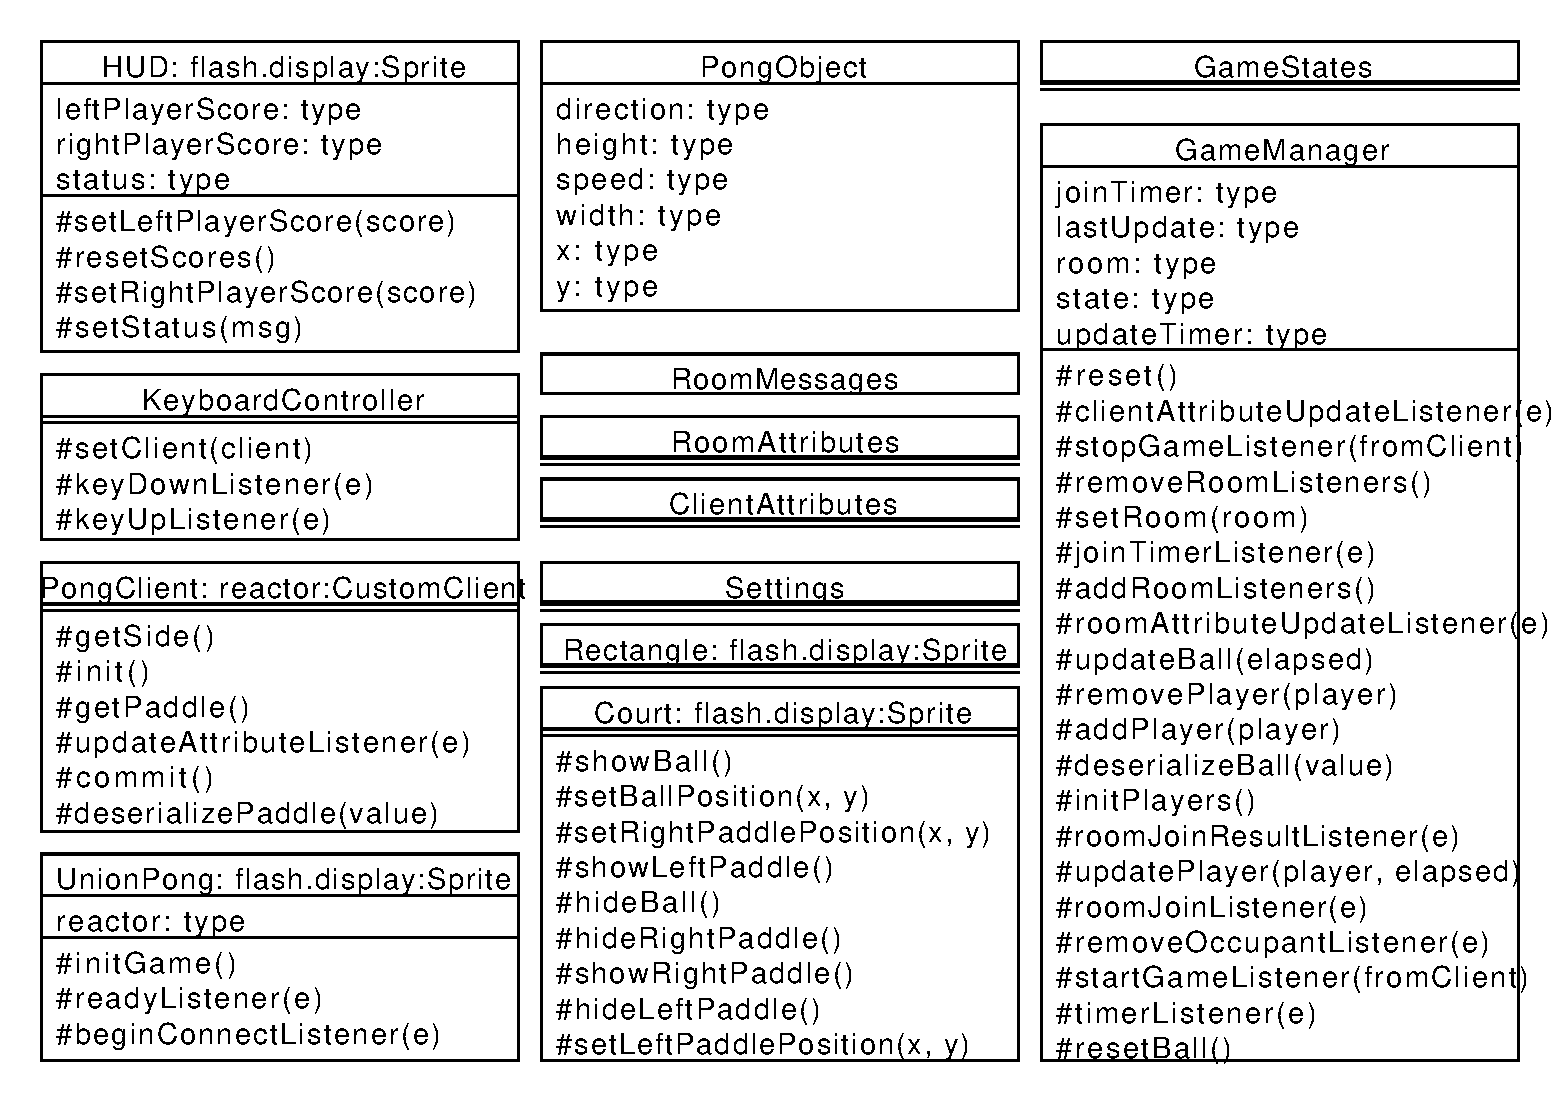
\includegraphics[scale=0.350000]{pics/UnionPong-manuallayout.pdf}
\caption{The 13 classes in UnionPong client side ActionScript.}
\end{figure}


\section{Discussion%
  \label{discussion}%
}


\subsection{Interpretation and validity of Object-Point data%
  \label{interpretation-and-validity-of-object-point-data}%
}

The fact that UnionPong obtains much higher OP values indicating a
more complex API does not mean that the Union platform would be
somehow inferior. Instead, it highlights the nature of game
development at a different abstraction level. As we discussed in
Section IV.B, the platforms achieve the basic functionality of the
Pong game, such as synchronizing object movements and ball collisions
and bounces, in different ways: UnionPong uses game specific messages,
whereas TundraPong relies on the built-in functionality of the Tundra
platform. Otherwise, the two APIs are very similar regarding
networking. Both have an abstract container for the state, a Room in
Union, and a Scene in Tundra. An application can store own custom
state information as special attributes in the container, and the
system takes care of automatically synchronizing changes to the state
information. Both use callbacks heavily, for example to listen to new
clients entering the service (an event of Room in Union's Reaktor and
in the RoomModule on the Union server separately, an event of the
Server core API object in Tundra server) and to attribute changes
received from the network. They both also allow sending simple ad-hoc
custom messages: Tundra uses them for game events such as informing of
a victory with the associated data; UnionPong uses them for
networking, including also paddle and ball movements, which Tundra
does automatically. These similarities indicate that the OP analysis
effectively captures the aforementioned differences in the scope and
the abstraction level of the platforms.

Looking at the OP data and considering the OP method, our
interpretation is that the OP method succeeds in illustrating the
difference in scope and abstraction level between the two
codebases. We have to ask whether the OP method does that better than
some other, perhaps simpler, metrics would do. From previous research
we know that the OP method does succeed in identifying complexity that
a simple LoC metric would miss. Our data seems to support that same
conclusion, as the LoC measure would give a even larger complexity
difference between the two implementations (115:565 for full
clients). Based on qualitative analysis, we think that the smaller
relative difference indicated by the OP data is more appropriate. Even
though UnionPong client needs to do more, and especially has many more
classes, most of the classes are very simple and most of the source
code is not very complex. Considering only static class information,
the difference would be even greater (27:180). TundraPong has
relatively long methods and a lot of function calls, which lead to
relative high MP count in the dynamic analysis (63:196). We think that
changes the final OP score to a realistic ratio (90:376).

Based on the OP data we cannot really say whether the tool and the OP
method misses something essential in the API complexity analysis. For
example, the OP method does not take into account anything specific to
networking: the need to think of connections, defining and sending
network messages etc. They are of course accounted for as normal data
definitions and function calls, but would some networking specific
metric, for example for the number of messages, be more useful
instead? Arguably, they present an additional complexity that the game
developer has to manage.


\subsection{Built-in platform logic vs. custom application logic%
  \label{built-in-platform-logic-vs-custom-application-logic}%
}

As TundraPong shows, implementing a game on an rich platform such as
Tundra can require a comparatively small amount of work. However,
custom game specific solutions for game object data, network messages,
movement inter/extrapolation and collisions can easily be more
powerful and even required. For example, if the game takes place on a
small spherical world, a mini planet, Tundra’s built-in euclidean
movement techniques become suddenly much less useful. Therefore, the
logic underlying the Union platform and other similar smaller
libraries is sound. Game developers often need custom solutions, so
the platform just provides the lower level tools for messaging and
stays out of the way for the rest. There is a caveat,
though. Optimizing and perfecting for example movement synchronization
is not trivial, thus it is often useful to have a mature shared
implementation. Tundra’s rigidbody movement messaging was recently
optimized, decreasing the message size from the 70 bytes/update of the
initial naive design to 11 bytes/update in the current version. So
having both reusable existing solutions and providing support for
custom messaging makes sense.  Tundra provides custom messaging in two
ways: high-level entity actions, used in the TundraPong game, and the
efficient low level custom messaging with the kNet library which is
used for the built-in functionality as well.

\subsection{Limitations of the study%
  \label{limitations-of-the-study}%
}

The Pong game used as the minimal reference of a networked multiplayer
game in this study is very simplistic. Much of the complexity of real
networked games, and especially large scale commercial MMOGs, lies in
areas not addressed by this study: service reliablity, availability,
restorability and scalability \cite{middleware}. Networked programming
in general is also typically complex due to the need to handle several
kinds of error situations, such as lost data, dropped connections and
conflicts from simultaneous actions. The Pong reference
implementations of this study may well be limited in that they do not
handle such issues in the way a production quality game must handle,
which probably increases the complexities. However, both Pong games
are built on very high-level networked game platforms, which strive to
hide the complexity of networking from the developer. Whether and how
they really achieve that cannot be determined from the data of this
study, but would require a different analysis.

In future work the shortcoming of relying on too simple reference
games in API complexity analysis could be addressed in two
ways. First, we could analyze the codebases of real production quality
games. However, typically a particular game exists only as a single
implementation, which prevents comparative analysis. Nevertheless, the
analysis could still provide valuable insight into assessing the
evolution of the complexity of the game, and the correlation of the
complexity with the monetary expenses of the development
effort. Second, we could develop a more complex reference game and
ensure its completeness. Such a reference game should be carefully
specified to cover all relevant areas of networked gaming, but still
remain small enough to allow implementation within a realistic
timeframe. Existing canonical implementations may provide a starting
point, as for example several commercial networked 3D first-person
shooter (FPS) games have been open sourced (Quake, Cube2), and at
least one highlevel platform already features a FPS as a tutorial
(Torque3D).


\section{Conclusion%
  \label{conclusion}%
}

We first presented a tool for the automated quantitative assessment of
the complexity of an API by extracting Sneed’s Object-Point data from
a source code using the API. We then compared the API complexity of
two platforms for developing networking games, by extracting the OP
data from two pre-existing implementations of the Pong game atop these
platforms with the tool. The OP data and the related UML diagrams
indicate that the tool successfully quantifies the different amounts
of complexity that the game developer has to cope with on these two
platforms. However, the difference in the relative complexity of the
APIs is very much due to the different underlying design rationale of
the platforms, the other relying on built-in functionality of the
platform and the other on custom application logic embedded in the
client.

In any case, automating data extraction for subsequent OP analysis
opens up fascinating opportunities for future work in platform and API
development. We could conduct longitudinal assessment of the evolution
of the complexity of a particular API and codebase over time, dissect
a software by running a series of OP analyses to pinpoint potential
sources of complexity, and compare networking stacks based on
different protocols for similar functionality.


\section{Downloads%
  \label{downloads}%
}

Our tool and the datasets used in this study are available online at
\url{https://github.com/realXtend/doc/tree/master/netgames/tools/}. The
work-in-progress executable is pointcounter.py that contains the
implementation of the Object-Point method.

\section*{Acknowledgements}

To be added.

\bibliography{IEEEabrv,bib}

\end{document}
